\documentclass[aspectratio=169,11pt]{beamer}

\usepackage[utf8]{inputenc}
\usepackage[T1]{fontenc}
\usepackage[french]{babel}
\usepackage{amsmath,amssymb}
\usepackage{newpxtext}
\usepackage{newpxmath}
\usepackage{booktabs,tabularx,array,multirow}
\usepackage{colortbl}
\usepackage{tikz}
\usepackage{pgfplots}
\pgfplotsset{compat=1.18}

\definecolor{marine}{HTML}{17365D}
\definecolor{bleuclair}{HTML}{EEF6FA}
\definecolor{or}{HTML}{18A99A}
\definecolor{bleuvif}{HTML}{2E64E8}
\definecolor{gris}{HTML}{F4F8FA}
\definecolor{orangeclimat}{HTML}{E98300}
\definecolor{bleugris}{HTML}{60748F}
\definecolor{vertfonce}{HTML}{176B3A}
\definecolor{jauneregime}{HTML}{C9A900}
\setbeamercolor{contextheading}{fg=marine,bg=marine!12}
\setbeamercolor{contextbody}{fg=marine,bg=gris}
\setbeamercolor{metricnavy}{fg=white,bg=marine}
\setbeamercolor{metricorange}{fg=white,bg=orangeclimat}
\setbeamercolor{metricgray}{fg=white,bg=bleugris}

\usetheme{default}
\usecolortheme{default}
\usefonttheme{serif}
\setbeamercolor{background canvas}{bg=bleuclair}
\setbeamercolor{normal text}{fg=marine,bg=bleuclair}
\setbeamercolor{structure}{fg=marine}
\setbeamercolor{frametitle}{fg=white,bg=marine}
\setbeamercolor{title}{fg=marine}
\setbeamercolor{block title}{fg=marine,bg=white}
\setbeamercolor{block body}{fg=marine,bg=white}
\setbeamercolor{block title alerted}{fg=marine,bg=white}
\setbeamercolor{block body alerted}{fg=marine,bg=white}
\setbeamercolor{alerted text}{fg=or}
\setbeamercolor{topbar}{fg=white,bg=marine}
\setbeamercolor{topbaraccent}{fg=white,bg=bleuvif}
\setbeamercolor{covercard}{fg=marine,bg=white}
\setbeamercolor{coverfooter}{fg=white,bg=marine}
\setbeamercolor{agendarow}{fg=marine,bg=white}
\setbeamercolor{pagenum}{fg=white,bg=marine}
\setbeamertemplate{blocks}[rounded][shadow=false]
\setbeamerfont{block title}{series=\bfseries,size=\small}
\setbeamertemplate{navigation symbols}{}
\setbeamertemplate{itemize item}{\color{or}\small$\blacktriangleright$}
\setbeamertemplate{enumerate item}{\color{marine}\insertenumlabel.}
\setbeamertemplate{footline}{%
  \begin{tikzpicture}[remember picture,overlay]
    \draw[or,line width=0.8pt] ([xshift=-0.58cm,yshift=0.62cm]current page.south east) circle (0.25cm);
    \draw[marine!55,line width=0.8pt] ([xshift=-0.31cm,yshift=0.48cm]current page.south east) circle (0.18cm);
  \end{tikzpicture}%
  \leavevmode\hbox to \paperwidth{\hfil%
    \colorbox{marine}{\makebox[0.48cm][c]{\color{white}\scriptsize\insertframenumber}}%
    \hfil}%
  \vskip0pt%
}
\setbeamertemplate{frametitle}{%
  \nointerlineskip%
  \begin{beamercolorbox}[wd=\paperwidth,ht=0.48cm,dp=0.20cm,leftskip=0.55cm]{frametitle}%
    \usebeamerfont{frametitle}\insertframetitle
  \end{beamercolorbox}%
  \nointerlineskip\hbox{\color{or}\rule{\paperwidth}{0.055cm}}%
  \vspace{0.10cm}%
}
\setbeamerfont{frametitle}{series=\bfseries,size=\small}
\setbeamersize{text margin left=6mm,text margin right=6mm}

\title[Variabilité pluviométrique au Sénégal]{Analyse des dynamiques climatiques et de leur variabilité en fonction de la pluviométrie au Sénégal}
\author{ZONGO Abdoul Kader}
\institute{École nationale de la Statistique et de l'Analyse économique Pierre Ndiaye (ENSAE)}
\date{Novembre 2026}

\begin{document}

% 1. Page de garde
\setbeamercolor{background canvas}{bg=white}
\begin{frame}[plain]
  \bfseries
  \vspace*{0cm}
  \begin{center}
    {\small\bfseries\color{marine}RÉPUBLIQUE DU SÉNÉGAL\par}
    \vspace{0.01cm}
    
\includegraphics[height=0.90cm,keepaspectratio]{armoiries_senegal.png}\par
    {\footnotesize Ministère de l’Économie des Finances et du Plan (MEFP)\par}
    {\tiny\bfseries\color{marine}**********\par}
    {\footnotesize Agence nationale de la Statistique et de la Démographie (ANSD)\par}
    
\includegraphics[height=0.78cm,keepaspectratio]{Logo_ANSD.png.jpg}\par
    {\tiny\bfseries\color{marine}********\par}
  \end{center}
  \vspace{-0.20cm}
  \begin{columns}[T,onlytextwidth]
    \column{0.48\textwidth}
      \centering
      {\footnotesize École nationale de la Statistique et de l’Analyse économique\\(ENSAE)}
    \column{0.48\textwidth}
      \centering
      {\footnotesize Direction de la Statistique Économique et de la Comptabilité nationale\\(DSECN)}
  \end{columns}
  \vspace{-0.20cm}
  \begin{center}
    \begin{tikzpicture}
      \node[draw=marine,line width=1.3pt,rounded corners=5pt,inner xsep=0.12cm,inner ysep=0.05cm,
        text width=0.72\textwidth,align=center] (titlebox) {{\color{marine}\fontsize{13}{15}\selectfont\bfseries Analyse des dynamiques climatiques\\[0.03cm]et de leur variabilité en fonction de la\\[0.03cm]pluviométrie au Sénégal}};
      \node[fill=bleugris,text=white,rounded corners=5pt,inner xsep=0.28cm,inner ysep=0.08cm,
        font=\footnotesize\bfseries] at ([yshift=0.18cm]titlebox.north) {SOUTENANCE DE RAPPORT DE STAGE};
    \end{tikzpicture}
  \end{center}
  \vspace{-0.20cm}
  \begin{columns}[T,onlytextwidth]
    \column{0.48\textwidth}
      \centering
      {\scriptsize\color{marine}Présenté par :\par}
      {\footnotesize\bfseries\color{marine}ZONGO Abdoul Kader\par}
      {\scriptsize Élève Ingénieur Statisticien Économiste}
    \column{0.48\textwidth}
      \centering
      {\scriptsize\color{marine}Encadré par :\par}
      {\footnotesize\bfseries\color{marine}M. Mouhamadou Bassirou DIOUF\par}
      {\scriptsize Comptable national}
  \end{columns}
  \vspace{-0.12cm}
  \begin{center}
    {\scriptsize\color{marine}Novembre 2026}
  \end{center}
\end{frame}
\setbeamercolor{background canvas}{bg=bleuclair}

% 2. Plan de la présentation
\begin{frame}[plain]
  \vspace{0.48cm}
  \begin{center}
    {\color{marine}\LARGE\bfseries Plan de la présentation\par}
    \vspace{0.12cm}
    {\color{or}\rule{0.24\linewidth}{1.5pt}\par}
  \end{center}
  \vspace{0.30cm}
  \begin{center}
    \begin{beamercolorbox}[wd=0.82\textwidth,ht=0.48cm,dp=0.14cm,leftskip=0.20cm,rounded=true]{agendarow}
      \colorbox{marine}{\color{white}\makebox[0.52cm][c]{\bfseries 01}}\hspace{0.35cm}Introduction
    \end{beamercolorbox}\vspace{0.06cm}
    \begin{beamercolorbox}[wd=0.82\textwidth,ht=0.48cm,dp=0.14cm,leftskip=0.20cm,rounded=true]{agendarow}
      \colorbox{marine}{\color{white}\makebox[0.52cm][c]{\bfseries 02}}\hspace{0.35cm}Données et méthodologie
    \end{beamercolorbox}\vspace{0.06cm}
    \begin{beamercolorbox}[wd=0.82\textwidth,ht=0.48cm,dp=0.14cm,leftskip=0.20cm,rounded=true]{agendarow}
      \colorbox{marine}{\color{white}\makebox[0.52cm][c]{\bfseries 03}}\hspace{0.35cm}Résultats
    \end{beamercolorbox}\vspace{0.06cm}
    \begin{beamercolorbox}[wd=0.82\textwidth,ht=0.48cm,dp=0.14cm,leftskip=0.20cm,rounded=true]{agendarow}
      \colorbox{marine}{\color{white}\makebox[0.52cm][c]{\bfseries 04}}\hspace{0.35cm}Discussion
    \end{beamercolorbox}\vspace{0.06cm}
    \begin{beamercolorbox}[wd=0.82\textwidth,ht=0.48cm,dp=0.14cm,leftskip=0.20cm,rounded=true]{agendarow}
      \colorbox{marine}{\color{white}\makebox[0.52cm][c]{\bfseries 05}}\hspace{0.35cm}Conclusion et recommandations
    \end{beamercolorbox}
  \end{center}
  \vfill
  \noindent\hfill
  \begin{tikzpicture}[baseline=0pt]
    \draw[or,line width=0.8pt] (0,0) circle (0.25cm);
    \draw[marine!55,line width=0.8pt] (0.27,-0.13) circle (0.18cm);
  \end{tikzpicture}
  \hspace{0.12cm}
\end{frame}

% 3. Contexte et justification (1/2)
\begin{frame}{Contexte et justification (1/2) : un climat qui change, une pluie qui varie}
  \begin{columns}[T,onlytextwidth]
    \column{0.54\textwidth}
      \begin{beamercolorbox}[wd=\linewidth,rounded=true,sep=0pt]{contextbody}
        \begin{beamercolorbox}[wd=\linewidth,ht=0.40cm,dp=0.08cm,leftskip=0.16cm]{contextheading}
          \bfseries Un enjeu climatique et hydrique
        \end{beamercolorbox}
        \begin{beamercolorbox}[wd=\linewidth,sep=0.08cm]{contextbody}
          \footnotesize
          \begin{itemize}
            \setlength\itemsep{0.10cm}
            \item Le changement climatique affecte le cycle de l'eau autant que les températures (GIEC, 2021).
            \item Sécheresses, inondations et disponibilité de l'eau influencent les écosystèmes et les activités humaines.
          \end{itemize}
        \end{beamercolorbox}
      \end{beamercolorbox}
      \vspace{0.20cm}
      \begin{beamercolorbox}[wd=\linewidth,rounded=true,sep=0pt]{contextbody}
        \begin{beamercolorbox}[wd=\linewidth,ht=0.40cm,dp=0.08cm,leftskip=0.16cm]{contextheading}
          \bfseries Le Sahel au cœur des variations
        \end{beamercolorbox}
        \begin{beamercolorbox}[wd=\linewidth,sep=0.08cm]{contextbody}
          \footnotesize
          \begin{itemize}
            \setlength\itemsep{0.10cm}
            \item Une rupture pluviométrique majeure est documentée autour de 1968-1972.
            \item Sa durée et le début de la reprise ont fait débat dans la littérature (Lamb, 1982 ; Nicholson, 1983 ; Le Barbé et Lebel, 1997 ; Ozer et al., 2003).
          \end{itemize}
        \end{beamercolorbox}
      \end{beamercolorbox}
    \column{0.42\textwidth}
      \begin{beamercolorbox}[wd=\linewidth,rounded=true,sep=0.10cm,center]{metricnavy}
        {\Large\bfseries 1968-1972\par}
        {\small Épisode déficitaire majeur documenté au Sahel}
      \end{beamercolorbox}
      \vspace{0.12cm}
      \begin{beamercolorbox}[wd=\linewidth,rounded=true,sep=0.10cm,center]{metricorange}
        {\Large\bfseries 117mm\par}
        {\small Dakar en 1972, contre une médiane de 500mm\\(Dacosta et al., 2002)}
      \end{beamercolorbox}
      \vspace{0.12cm}
      \begin{beamercolorbox}[wd=\linewidth,rounded=true,sep=0.10cm,center]{metricgray}
        {\Large\bfseries Depuis 2000\par}
        {\small Reprise des cumuls, partielle et non uniforme (GAYE, 2017)}
      \end{beamercolorbox}
  \end{columns}
\end{frame}

% 4. Contexte et justification (2/2)
\begin{frame}{Contexte et justification (2/2) : pourquoi cette étude ?}
  \begin{columns}[T,onlytextwidth]
    \column{0.54\textwidth}
      \begin{beamercolorbox}[wd=\linewidth,rounded=true,sep=0pt]{contextbody}
        \begin{beamercolorbox}[wd=\linewidth,ht=0.40cm,dp=0.08cm,leftskip=0.16cm]{contextheading}
          \bfseries Un pays exposé
        \end{beamercolorbox}
        \begin{beamercolorbox}[wd=\linewidth,sep=0.08cm]{contextbody}
          \footnotesize
          \begin{itemize}
            \setlength\itemsep{0.04cm}
            \item Situé à l’extrémité occidentale du Sahel, le Sénégal dépend fortement des précipitations.
            \item Il passe du domaine sahélien (Nord) au domaine soudano-guinéen (Sud).
            \item Les cumuls moyens vont de 271mm (Saint-Louis) à 1\,340mm (Ziguinchor).
          \end{itemize}
        \end{beamercolorbox}
      \end{beamercolorbox}
      \vspace{0cm}
      \begin{beamercolorbox}[wd=\linewidth,rounded=true,sep=0pt]{contextbody}
        \begin{beamercolorbox}[wd=\linewidth,ht=0.40cm,dp=0.08cm,leftskip=0.16cm]{contextheading}
          \bfseries Un manque dans la littérature
        \end{beamercolorbox}
        \begin{beamercolorbox}[wd=\linewidth,sep=0.01cm]{contextbody}
          \footnotesize
          \begin{itemize}
            \setlength\itemsep{0cm}
            \setlength\topsep{0pt}
            \setlength\parsep{0pt}
            \item Travaux souvent isolés : stations ou bassins versants.
            \item Pas de lectures conjointes des 14 régions.
            \item Tests univariés repèrent ruptures et tendances ; l’analyse multivariée relie les régions entre elles.
          \end{itemize}
        \end{beamercolorbox}
      \end{beamercolorbox}
    \column{0.42\textwidth}
      \begin{beamercolorbox}[wd=\linewidth,rounded=true,sep=0pt]{contextbody}
        \begin{beamercolorbox}[wd=\linewidth,ht=0.40cm,dp=0.08cm,leftskip=0.16cm]{contextheading}
          \small\bfseries Utilité pour la statistique publique
        \end{beamercolorbox}
        \begin{beamercolorbox}[wd=\linewidth,sep=0.14cm]{contextbody}
          \small
          Mieux documenter \textcolor{marine}{quand} et \textcolor{marine}{où} le régime pluviométrique évolue aide à éclairer :
          \vspace*{0.10cm}
          \begin{itemize}
            \setlength\itemsep{0.12cm}
            \item le suivi des statistiques environnementales ;
            \item la contextualisation des séries économiques sensibles au climat ;
            \item la planification agricole et hydrique, en croisant ces résultats avec les données sectorielles.
          \end{itemize}
        \end{beamercolorbox}
      \end{beamercolorbox}
  \end{columns}
\end{frame}

% 5. Problématique
\begin{frame}{Problématique}
  \vspace{0.18cm}
  \begin{center}
    \begin{beamercolorbox}[wd=0.90\textwidth,rounded=true,sep=0.28cm,center]{metricnavy}
    {\Large Comment la pluviométrie a-t-elle évolué au Sénégal au cours du temps,\\
    et quelle forme prend sa variabilité ?}
  \end{beamercolorbox}
  \end{center}
  \vspace{0.55cm}
  \begin{columns}[T,onlytextwidth]
    \column{0.31\textwidth}
      \uncover<1->{%
        \begin{beamercolorbox}[wd=\linewidth,rounded=true,sep=0pt]{contextbody}
          \begin{beamercolorbox}[wd=\linewidth,ht=0.40cm,dp=0.08cm,leftskip=0.14cm]{contextheading}
            \bfseries Question 1
          \end{beamercolorbox}
          \begin{beamercolorbox}[wd=\linewidth,sep=0.14cm]{contextbody}
            \footnotesize À quelles dates se situent les ruptures régionales, et quelle est leur ampleur ?
          \end{beamercolorbox}
        \end{beamercolorbox}
      }%
    \column{0.31\textwidth}
      \uncover<1->{%
        \begin{beamercolorbox}[wd=\linewidth,rounded=true,sep=0pt]{contextbody}
          \begin{beamercolorbox}[wd=\linewidth,ht=0.40cm,dp=0.08cm,leftskip=0.14cm]{contextheading}
            \bfseries Question 2
          \end{beamercolorbox}
          \begin{beamercolorbox}[wd=\linewidth,sep=0.14cm]{contextbody}
            \footnotesize Quelles sont les principales structures de variabilité pluviométrique entre les régions ?
          \end{beamercolorbox}
        \end{beamercolorbox}
      }%
    \column{0.31\textwidth}
      \uncover<1->{%
        \begin{beamercolorbox}[wd=\linewidth,rounded=true,sep=0pt]{contextbody}
          \begin{beamercolorbox}[wd=\linewidth,ht=0.40cm,dp=0.08cm,leftskip=0.14cm]{contextheading}
            \bfseries Question 3
          \end{beamercolorbox}
          \begin{beamercolorbox}[wd=\linewidth,sep=0.14cm]{contextbody}
            \footnotesize Quels régimes pluviométriques caractérisent le pays, et comment les années s'y répartissent-elles ?
          \end{beamercolorbox}
        \end{beamercolorbox}
      }%
  \end{columns}
\end{frame}

% 6. Objectifs
\begin{frame}{Objectifs de l'étude}
  \begin{tikzpicture}[remember picture,overlay]
    \node[fill=marine,text=white,rounded corners=9pt,align=center,text width=0.78\paperwidth,minimum height=1.20cm,inner sep=7pt] (objectifgeneral)
      at ([yshift=-1.97cm]current page.north)
      {{\large\bfseries Objectif général\par}\vspace{2pt}\normalsize Analyser l’évolution de la pluviométrie\\[2pt]au Sénégal et caractériser sa variabilité};
    \node<1->[fill=orangeclimat!14,draw=orangeclimat,line width=0.8pt,text=marine,rounded corners=8pt,align=center,text width=0.25\paperwidth,minimum height=2.70cm,inner sep=6pt] (objectifun)
      at ([xshift=-5.00cm,yshift=-5.60cm]current page.north)
      {{\large\bfseries OS1\par}\vspace{3pt}\footnotesize Identifier les\\ruptures dans les\\séries pluviométriques\\régionales et en\\mesurer l’ampleur};
    \draw<1->[->,marine,line width=1pt] (objectifgeneral.south) -- (objectifun.north);
    \node<1->[fill=orangeclimat!14,draw=orangeclimat,line width=0.8pt,text=marine,rounded corners=8pt,align=center,text width=0.25\paperwidth,minimum height=2.70cm,inner sep=6pt] (objectifdeux)
      at ([yshift=-5.60cm]current page.north)
      {{\large\bfseries OS2\par}\vspace{3pt}\footnotesize Dégager les\\principales structures\\de variabilité entre\\les régions};
    \draw<1->[->,marine,line width=1pt] (objectifgeneral.south) -- (objectifdeux.north);
    \node<1->[fill=orangeclimat!14,draw=orangeclimat,line width=0.8pt,text=marine,rounded corners=8pt,align=center,text width=0.25\paperwidth,minimum height=2.70cm,inner sep=6pt] (objectiftrois)
      at ([xshift=5.00cm,yshift=-5.60cm]current page.north)
      {{\large\bfseries OS3\par}\vspace{3pt}\scriptsize Mettre en évidence\\les grands régimes\\pluviométriques du pays\\en y classant\\les années};
    \draw<1->[->,marine,line width=1pt] (objectifgeneral.south) -- (objectiftrois.north);
  \end{tikzpicture}
  \vspace{6.50cm}
\end{frame}

% 7. Hypothèses
\begin{frame}{Hypothèses de recherche}
  \begin{tikzpicture}[remember picture,overlay]
    \node[fill=gris,rounded corners=2pt,minimum width=1.45cm,minimum height=5.00cm,inner sep=0pt]
      at ([xshift=-6.35cm,yshift=-4.43cm]current page.north) {};
    \node[font=\rmfamily\large\bfseries,text=marine] at ([xshift=-6.35cm,yshift=-2.55cm]current page.north) {H1};
    \node[font=\rmfamily\large\bfseries,text=marine] at ([xshift=-6.35cm,yshift=-3.81cm]current page.north) {H2};
    \node[font=\rmfamily\large\bfseries,text=marine] at ([xshift=-6.35cm,yshift=-5.07cm]current page.north) {H3};
    \node[font=\rmfamily\large\bfseries,text=marine] at ([xshift=-6.35cm,yshift=-6.33cm]current page.north) {H4};

    \node[anchor=west,align=left,text width=9.65cm,inner sep=0pt] at ([xshift=-5.35cm,yshift=-2.55cm]current page.north)
      {\rmfamily\large Les séries pluviométriques régionales présentent au moins une \textcolor{marine}{rupture} statistiquement \mbox{significative}.};
    \node[anchor=west,align=left,text width=9.65cm,inner sep=0pt] at ([xshift=-5.35cm,yshift=-3.81cm]current page.north)
      {\rmfamily\large Les moyennes \textcolor{marine}{avant et après} rupture diffèrent \mbox{significativement}.};
    \node[anchor=west,align=left,text width=9.65cm,inner sep=0pt] at ([xshift=-5.35cm,yshift=-5.07cm]current page.north)
      {\rmfamily\large Les régimes pluviométriques traduisent une \textcolor{marine}{\mbox{hétérogénéité} \mbox{spatiale}} entre régions.};
    \node[anchor=west,align=left,text width=9.65cm,inner sep=0pt] at ([xshift=-5.35cm,yshift=-6.33cm]current page.north)
      {\rmfamily\large Une typologie cohérente des années \textcolor{marine}{sèches, humides et de \mbox{transition}} se dégage.};

    \node[anchor=west,text width=2.0cm,inner sep=0pt] at ([xshift=5.05cm,yshift=-2.55cm]current page.north)
      {\rmfamily\large $\rightarrow$ OS1};
    \node[anchor=west,text width=2.0cm,inner sep=0pt] at ([xshift=5.05cm,yshift=-3.81cm]current page.north)
      {\rmfamily\large $\rightarrow$ OS1};
    \node[anchor=west,text width=2.0cm,inner sep=0pt] at ([xshift=5.05cm,yshift=-5.07cm]current page.north)
      {\rmfamily\large $\rightarrow$ OS2};
    \node[anchor=west,text width=2.0cm,inner sep=0pt] at ([xshift=5.05cm,yshift=-6.33cm]current page.north)
      {\rmfamily\large $\rightarrow$ OS3};
  \end{tikzpicture}
\end{frame}

% 8. Données
\begin{frame}{Données et méthodologie(1/4) : présentation des données}
  \begin{columns}[T,onlytextwidth]
    \column{0.48\textwidth}
      \begin{block}{Source et contenu}
        \small
        \begin{itemize}
          \item Source : ANACIM.
          \item Cumuls pluviométriques annuels en millimètres.
          \item Quatorze séries régionales, une série par région.
        \end{itemize}
      \end{block}
    \column{0.48\textwidth}
      \begin{block}{Période et couverture}
        \small
        \begin{itemize}
          \item Période commune : 1961-2025, soit 65 années.
          \item Aucune valeur manquante sur la période retenue.
          \item Couverture des quatorze régions du Sénégal.
          \item Séries annuelles agrégées, sans détail infra-annuel.
        \end{itemize}
      \end{block}
  \end{columns}
\end{frame}

% 9. Méthodologie : chaîne d’analyse
\begin{frame}{Données et méthodologie(2/4) : démarche d’ensemble}
  \centering
  \vspace{0.28cm}
  \begin{tikzpicture}[
    node distance=0cm,
    process/.style={
      draw=marine,
      line width=0.75pt,
      rounded corners=3pt,
      fill=gris,
      text=marine,
      text width=2.95cm,
      minimum height=1.72cm,
      align=center,
      inner sep=5pt,
      font=\small
    },
    firststep/.style={process,fill=marine,text=white},
    flow/.style={->,draw=marine,line width=0.9pt}
  ]
    \node[firststep] (donnees) at (-4.4,1.15)
      {\textbf{Données}\\14 séries, 1961-2025};
    \node[process] (verification) at (0,1.15)
      {\textbf{Vérifications préalables}\\Autocorrélation, tendance,\\variances, normalité};
    \node[process] (ruptures) at (4.4,1.15)
      {\textbf{Détection de ruptures}\\4 procédures + règle de majorité};

    \node[process] (cah) at (-4.4,-1.25)
      {\textbf{CAH (Ward)}\\Sur les axes retenus};
    \node[process] (acp) at (0,-1.25)
      {\textbf{ACP réduite}\\14 séries centrées-réduites};
    \node[process] (moyennes) at (4.4,-1.25)
      {\textbf{Moyennes avant/après}\\Student ou Welch};

    \draw[flow] (donnees.east) -- (verification.west);
    \draw[flow] (verification.east) -- node[above,font=\scriptsize\itshape,text=marine,fill=bleuclair,inner sep=1pt] {Temps} (ruptures.west);
    \draw[flow] (ruptures.south) -- (moyennes.north);
    \draw[flow] (moyennes.west) -- node[below,font=\scriptsize\itshape,text=marine,fill=bleuclair,inner sep=1pt] {Espace} (acp.east);
    \draw[flow] (acp.west) -- node[below,font=\scriptsize\itshape,text=marine,fill=bleuclair,inner sep=1pt] {Régimes} (cah.east);
  \end{tikzpicture}
\end{frame}

% 10. Méthodes statistiques
\begin{frame}{Données et méthodologie(3/4) : détecter, valider et mesurer l’ampleur d’une rupture}
  \small
  \begin{columns}[T,onlytextwidth]
    \column{0.55\textwidth}
      \begin{beamercolorbox}[wd=\linewidth,rounded=true,sep=0pt]{contextbody}
        \begin{beamercolorbox}[wd=\linewidth,ht=0.42cm,dp=0.08cm,leftskip=0.16cm]{contextheading}
          \bfseries Quatre procédures complémentaires
        \end{beamercolorbox}
        \begin{beamercolorbox}[wd=\linewidth,sep=0.10cm]{contextbody}
          \footnotesize
          \begin{itemize}
            \setlength\itemsep{0.07cm}
            \item \textbf{Pettitt (1979)} : date au maximum de $|U_t|$.
            \item \textbf{Buishand (1982)} : date au maximum de $|S_k^*|$.
            \item \textbf{Lee--Heghinian (1977)} : approche bayésienne, mode a posteriori (pas de seuil).
            \item \textbf{Hubert et al. (1989)} : segmentation (Scheffé, 1\%) ; premier point de rupture retenu.
          \end{itemize}
        \end{beamercolorbox}
      \end{beamercolorbox}
    \column{0.43\textwidth}
      \begin{beamercolorbox}[wd=\linewidth,rounded=true,sep=0pt]{contextbody}
        \begin{beamercolorbox}[wd=\linewidth,ht=0.42cm,dp=0.08cm,leftskip=0.16cm]{contextheading}
          {\color{marine}\bfseries Règle de majorité}
        \end{beamercolorbox}
        \begin{beamercolorbox}[wd=\linewidth,sep=0.10cm]{contextbody}
          \small
          Rupture \textcolor{marine}{avérée} si au moins 3 procédures sur 4 proposent une date à $\pm 3$ ans.
        \end{beamercolorbox}
      \end{beamercolorbox}
      \vspace{0.14cm}
      \begin{beamercolorbox}[wd=\linewidth,rounded=true,sep=0pt]{contextbody}
        \begin{beamercolorbox}[wd=\linewidth,ht=0.42cm,dp=0.08cm,leftskip=0.16cm]{contextheading}
          \bfseries Robustesse
        \end{beamercolorbox}
        \begin{beamercolorbox}[wd=\linewidth,sep=0.10cm]{contextbody}
          \small
          Analyse de sensibilité de la tolérance de 0 à 5 ans (annexe F) : \textcolor{marine}{8 régions} pour 0 à 3 ans ; 10 pour 4-5 ans (Kolda et Thiès).
        \end{beamercolorbox}
      \end{beamercolorbox}
  \end{columns}
  \vspace{0.14cm}
  \begin{columns}[T,onlytextwidth]
    \column{0.49\textwidth}
      \begin{beamercolorbox}[wd=\linewidth,rounded=true,sep=0pt]{contextbody}
        \begin{beamercolorbox}[wd=\linewidth,ht=0.42cm,dp=0.08cm,leftskip=0.16cm]{contextheading}
          \bfseries Vérifications préalables
        \end{beamercolorbox}
        \begin{beamercolorbox}[wd=\linewidth,sep=0.10cm]{contextbody}
          \footnotesize
          Autocorrélation d’ordre 1 ($|r_1|<0{,}243$), Mann--Kendall et pente de Sen, Levene, Shapiro--Wilk.
        \end{beamercolorbox}
      \end{beamercolorbox}
    \column{0.49\textwidth}
      \begin{beamercolorbox}[wd=\linewidth,rounded=true,sep=0pt]{contextbody}
        \begin{beamercolorbox}[wd=\linewidth,ht=0.42cm,dp=0.08cm,leftskip=0.16cm]{contextheading}
          \bfseries Mesurer l'ampleur
        \end{beamercolorbox}
        \begin{beamercolorbox}[wd=\linewidth,sep=0.10cm]{contextbody}
          \footnotesize
          Comparaison avant/après : test de Student ou de Welch selon Levene.
        \end{beamercolorbox}
      \end{beamercolorbox}
  \end{columns}
\end{frame}

% 11. Méthodes multivariées et indice pluviométrique
\begin{frame}{Données et méthodologie(4/4) : structure spatiale et régimes}
  \small
  \begin{columns}[T,onlytextwidth]
    \column{0.49\textwidth}
      \begin{beamercolorbox}[wd=\linewidth,rounded=true,sep=0pt]{contextbody}
        \begin{beamercolorbox}[wd=\linewidth,ht=0.42cm,dp=0.08cm,leftskip=0.16cm]{contextheading}
          \bfseries ACP réduite
        \end{beamercolorbox}
        \begin{beamercolorbox}[wd=\linewidth,sep=0.08cm]{contextbody}
          \footnotesize
          \begin{itemize}
            \setlength\itemsep{0.06cm}
            \item Tableau de 65 années $\times$ 14 régions, séries centrées-réduites.
            \item Diagonalisation de la matrice de corrélation.
            \item Axes retenus selon le critère de Kaiser ($\lambda>1$).
          \end{itemize}
        \end{beamercolorbox}
      \end{beamercolorbox}
      \vspace{0.14cm}
      \begin{beamercolorbox}[wd=\linewidth,rounded=true,sep=0pt]{contextbody}
        \begin{beamercolorbox}[wd=\linewidth,ht=0.42cm,dp=0.08cm,leftskip=0.16cm]{contextheading}
          \bfseries CAH
        \end{beamercolorbox}
        \begin{beamercolorbox}[wd=\linewidth,sep=0.08cm]{contextbody}
          \footnotesize
          \begin{itemize}
            \setlength\itemsep{0.06cm}
            \item Classification sur les coordonnées des axes retenus.
            \item Distance euclidienne et critère de Ward.
            \item Trois classes fixées a priori : sèche, normale et humide.
          \end{itemize}
        \end{beamercolorbox}
      \end{beamercolorbox}
    \column{0.49\textwidth}
      \begin{beamercolorbox}[wd=\linewidth,rounded=true,sep=0pt]{contextbody}
        \begin{beamercolorbox}[wd=\linewidth,ht=0.42cm,dp=0.08cm,leftskip=0.16cm]{contextheading}
          \bfseries Indice pluviométrique standardisé (IPS)
        \end{beamercolorbox}
        \begin{beamercolorbox}[wd=\linewidth,sep=0.08cm]{contextbody}
          \footnotesize
          \begin{itemize}
            \setlength\itemsep{0.06cm}
            \item $\mathrm{IPS}_i=\dfrac{x_i-\bar{x}}{s}$ (Lamb, 1982).
            \item Lissage par filtre passe-bas de Hanning d’ordre 2 (poids : 0,06 ; 0,25 ; 0,38 ; 0,25 ; 0,06).
            \item Usage visuel uniquement : les tests portent sur les séries brutes.
          \end{itemize}
        \end{beamercolorbox}
      \end{beamercolorbox}
      \vspace{0.14cm}
      \begin{beamercolorbox}[wd=\linewidth,rounded=true,sep=0pt]{contextbody}
        \begin{beamercolorbox}[wd=\linewidth,ht=0.42cm,dp=0.08cm,leftskip=0.16cm]{contextheading}
          \bfseries Outils
        \end{beamercolorbox}
        \begin{beamercolorbox}[wd=\linewidth,sep=0.08cm]{contextbody}
          \footnotesize
          Python (scipy, statsmodels, scikit-learn) ; implémentation des tests réalisée en Python.
        \end{beamercolorbox}
      \end{beamercolorbox}
  \end{columns}
  \vspace{-0.12cm}
\end{frame}

% 11. Résultats : évolution de l'IPS moyen
\begin{frame}{Résultats (1/9) : l’IPS moyen révèle trois phases}
  \begin{columns}[T,onlytextwidth]
    \column{0.64\textwidth}
      \begin{tikzpicture}
        \begin{axis}[
          width=7.1cm,
          height=4.5cm,
          xmin=1961, xmax=2025,
          ymin=-2, ymax=2,
          xlabel={Année},
          ylabel={Indice pluviométrique standardisé moyen},
          label style={font=\scriptsize},
          tick label style={font=\tiny},
          xtick={1961,1969,1977,1985,1993,2001,2009,2017,2025},
          xticklabel style={rotate=45,anchor=east},
          xticklabel={\pgfmathprintnumber[1000 sep={}]{\tick}},
          ytick={-2,-1.5,...,2},
          yticklabel={\pgfmathprintnumber[use comma]{\tick}},
          axis lines=left,
          axis line style={draw=marine!65},
          tick align=outside,
          ymajorgrids=true,
          grid style={draw=marine!12},
          scale only axis,
          clip=true
        ]
          \addplot[or!65,thin,dashed,forget plot] coordinates {(1961,0) (2025,0)};
          \addplot[marine,line width=1.25pt,no marks] coordinates {
            (1961,0.713427431) (1962,0.536495259) (1963,0.765751755) (1964,1.100118867)
            (1965,0.822302312) (1966,1.080263991) (1967,1.098055156) (1968,-1.010273268)
            (1969,1.637914004) (1970,-0.544899817) (1971,0.335790056) (1972,-1.191535002)
            (1973,-0.590652491) (1974,0.009302538) (1975,0.40603287) (1976,-0.336231415)
            (1977,-1.286416777) (1978,0.197519145) (1979,-0.422294883) (1980,-1.045242313)
            (1981,-0.009275831) (1982,-0.803851743) (1983,-1.55625015) (1984,-0.755848965)
            (1985,-0.37245749) (1986,-0.533389885) (1987,-0.257647589) (1988,0.298816906)
            (1989,0.196158106) (1990,-0.82990673) (1991,-0.981306019) (1992,-0.911466325)
            (1993,-0.289250768) (1994,0.138397075) (1995,-0.488736819) (1996,-0.710935355)
            (1997,-0.443432106) (1998,-0.556160004) (1999,0.90149438) (2000,0.467202361)
            (2001,-0.204038225) (2002,-0.861968899) (2003,0.284404516) (2004,-0.178031021)
            (2005,0.709536362) (2006,-0.143051296) (2007,-0.54374981) (2008,0.547284554)
            (2009,0.438269277) (2010,1.425076065) (2011,-0.323640095) (2012,0.896015993)
            (2013,0.330766814) (2014,-0.978255049) (2015,0.582408023) (2016,0.140316651)
            (2017,-0.013181736) (2018,-0.488475913) (2019,-0.104403192) (2020,1.336376118)
            (2021,0.057531169) (2022,1.207437219) (2023,0.36392781) (2024,0.332631621)
            (2025,0.409232577)
          };
        \end{axis}
      \node[anchor=west,font=\scriptsize\itshape,text=marine] at ([xshift=0.25cm,yshift=-0.05cm]current bounding box.south west) {Source : ANACIM, calculs de l’auteur.};
      \end{tikzpicture}
    \column{0.34\textwidth}
      \vspace{0.30cm}
      \begin{beamercolorbox}[wd=\linewidth,rounded=true,sep=0.14cm]{contextbody}
        {\bfseries 1961-1969 :}\quad phase humide\par
        Pic de {\color{marine}\bfseries $+1{,}6$} en 1969.
      \end{beamercolorbox}
      \vspace{0.18cm}
      \begin{beamercolorbox}[wd=\linewidth,rounded=true,sep=0.14cm]{contextbody}
        {\bfseries 1970-2007 :}\quad déficit prolongé\par
        Minimum de {\color{marine}\bfseries $-1{,}7$} en 1983.
      \end{beamercolorbox}
      \vspace{0.18cm}
      \begin{beamercolorbox}[wd=\linewidth,rounded=true,sep=0.14cm]{contextbody}
        {\bfseries Depuis la fin des années 2000 :}\quad reprise\par
        Pics en 2009, 2013 et 2021 : {\color{marine}\bfseries $+1{,}3$ à $+1{,}4$}.
      \end{beamercolorbox}
  \end{columns}
\end{frame}

% 12. Résultats : vérifications préalables
\begin{frame}{Résultats (2/9) : vérifications préalables}
  \small
  \begin{columns}[T,onlytextwidth]
    \column{0.47\textwidth}
      \begin{beamercolorbox}[wd=\linewidth,rounded=true,sep=0pt]{contextbody}
        \begin{beamercolorbox}[wd=\linewidth,sep=0.09cm]{contextheading}
          \bfseries 12 régions sur 14 respectent les quatre hypothèses
        \end{beamercolorbox}
        \begin{beamercolorbox}[wd=\linewidth,sep=0.10cm]{contextbody}
          \footnotesize
          Indépendance, absence de tendance, homoscédasticité et normalité.
        \end{beamercolorbox}
      \end{beamercolorbox}
    \column{0.49\textwidth}
      \begin{beamercolorbox}[wd=\linewidth,rounded=true,sep=0pt]{contextbody}
        \begin{beamercolorbox}[wd=\linewidth,sep=0.09cm]{contextheading}
          {\color{marine}\bfseries Deux anomalies}
        \end{beamercolorbox}
        \begin{beamercolorbox}[wd=\linewidth,sep=0.08cm]{contextbody}
          \footnotesize
          \begin{itemize}
            \setlength\itemsep{0.04cm}
            \item \textbf{Kaolack} : tendance monotone ($Z=2{,}09$ ; $p=0{,}04$ ; pente de Sen $+2{,}49$ mm/an).
            \item \textbf{Matam} : autocorrélation ($r_1=0{,}32>0{,}243$).
          \end{itemize}
        \end{beamercolorbox}
      \end{beamercolorbox}
  \end{columns}
  \vspace{0.20cm}
  \begin{beamercolorbox}[wd=\textwidth,rounded=true,sep=0pt]{contextbody}
    \begin{beamercolorbox}[wd=\linewidth,sep=0.08cm]{contextheading}
      \bfseries Pourquoi c’est important ?
    \end{beamercolorbox}
    \begin{beamercolorbox}[wd=\linewidth,sep=0.10cm]{contextbody}
      \footnotesize
      Une tendance progressive ou une autocorrélation peuvent être confondues avec une rupture brutale (Pettitt, Buishand) ; ces deux régions sont donc interprétées avec prudence.
    \end{beamercolorbox}
  \end{beamercolorbox}
\end{frame}

% 13. Résultats : validation des ruptures
\begin{frame}{Résultats (3/9) : huit régions sur quatorze avec rupture avérée}
  \centering
  \vspace{0.22cm}
  \scriptsize
  \renewcommand{\arraystretch}{1.24}
  \setlength{\tabcolsep}{4pt}
  \begin{tabularx}{0.94\textwidth}{@{}>{\raggedright\arraybackslash}p{2.2cm}*{4}{>{\centering\arraybackslash}X}>{\centering\arraybackslash}p{0.9cm}>{\centering\arraybackslash}p{1.15cm}@{}}
    \toprule
    \textbf{Région} & \textbf{Pettitt} & \textbf{Buishand} & \textbf{Lee--H.} & \textbf{Hubert} & \textbf{Tests} & \textbf{Rupture} \\
    \midrule
    \rowcolor{marine!8}
    \textbf{Kédougou} & 1966 & 1966 & 1966 & 1966 & 4 & \textbf{1966} \\
    \textbf{Dakar} & 2004 & 1969 & 1969 & 1969 & 3 & \textbf{1969} \\
    \rowcolor{marine!8}
    \textbf{Saint-Louis} & 1997 & 1969 & 1969 & 1969 & 3 & \textbf{1969} \\
    \textbf{Sédhiou} & 2002 & 1969 & 1969 & 1969 & 3 & \textbf{1969} \\
    \rowcolor{marine!8}
    \textbf{Diourbel} & 1971 & 1971 & 1971 & 1971 & 4 & \textbf{1971} \\
    \textbf{Kaffrine} & 1998 & 1998 & 1998 & 1998 & 4 & \textbf{1998} \\
    \rowcolor{marine!8}
    \textbf{Fatick} & 2007 & 2007 & 2007 & 1971 & 3 & \textbf{2007} \\
    \textbf{Ziguinchor} & 2004 & 2007 & 2007 & 2007 & 4 & \textbf{2007} \\
    \midrule
    \rowcolor{gris}
    \multicolumn{1}{@{}l}{Kaolack, Kolda, Louga, Matam, Tamba., Thiès} & \multicolumn{4}{c}{Dates dispersées} & 2 & non avérée \\
    \bottomrule
  \end{tabularx}
  \vspace{0.18cm}

  {\footnotesize Règle : au moins 3 procédures sur 4 à $\pm 3$ ans. Kolda et Thiès deviennent avérées à $\pm 4$ ans (cas limites).\par}
  \vspace{0.08cm}
  {\scriptsize\itshape Source : ANACIM, calculs de l’auteur.}
\end{frame}

% 14. Résultats : deux profils de rupture
\begin{frame}{Résultats (4/9) : deux groupes de ruptures, deux visages}
  \centering
  \begin{columns}[T,onlytextwidth]
    \column{0.49\textwidth}
      \centering
      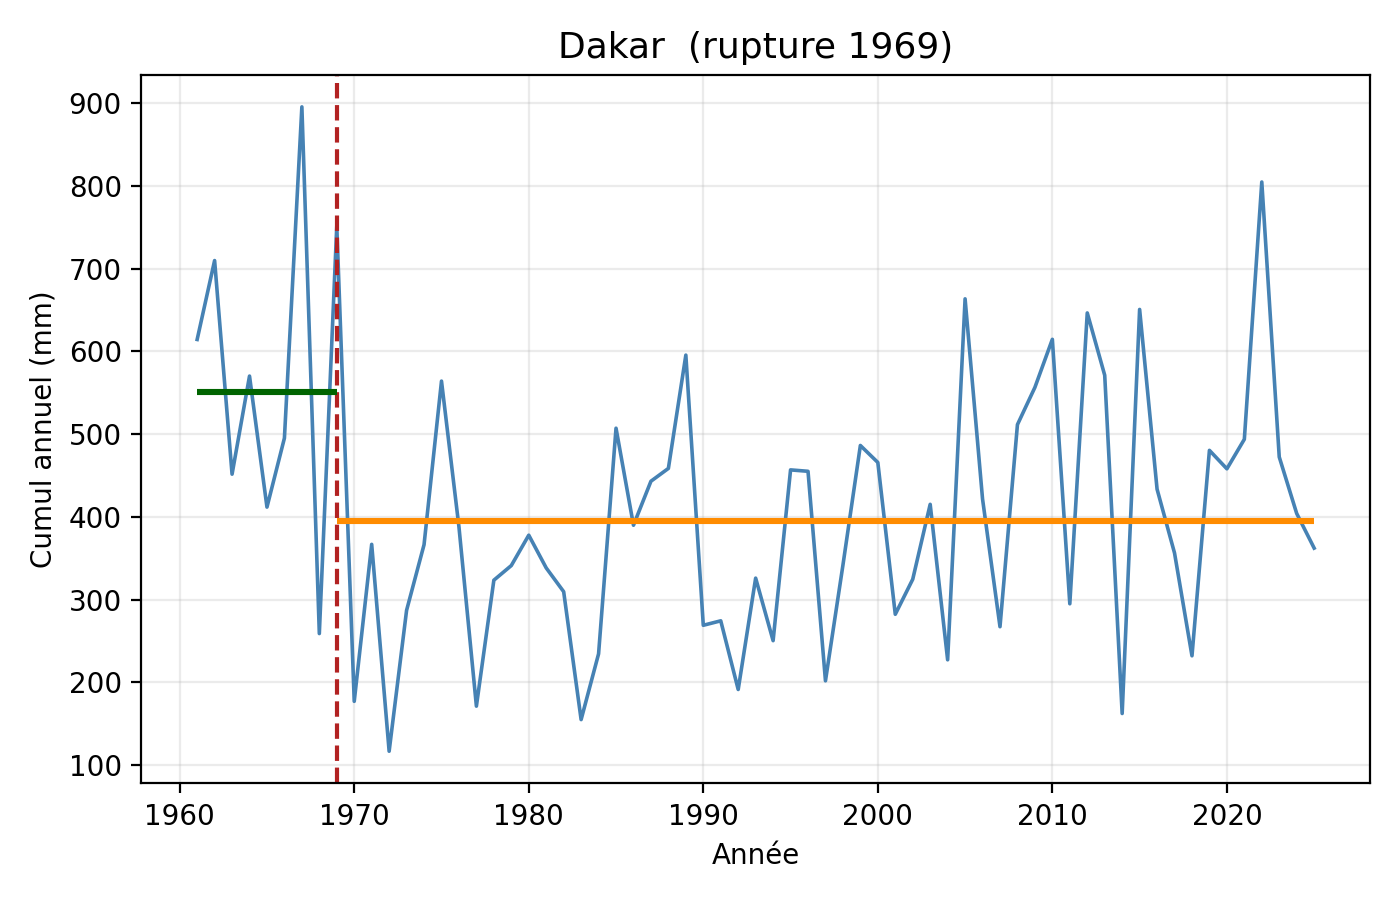
\includegraphics[width=\linewidth,height=4.4cm,keepaspectratio]{figures_individuelles_14stations/Dakar.png}
    \column{0.49\textwidth}
      \centering
      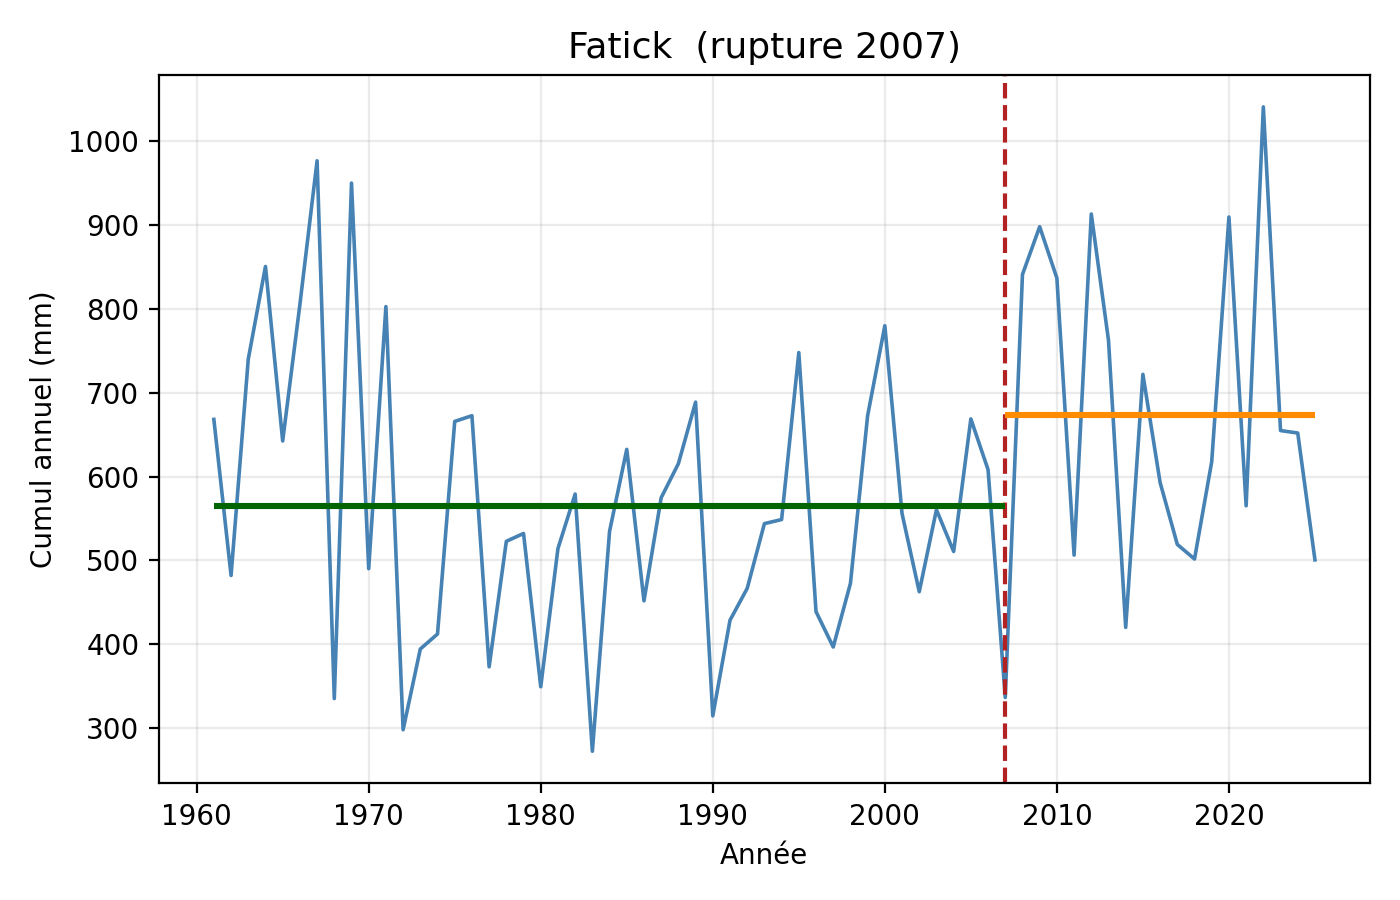
\includegraphics[width=\linewidth,height=4.4cm,keepaspectratio]{figures_individuelles_14stations/Fatick.png}
  \end{columns}
  \vspace{0.06cm}
  {\scriptsize Vert : moyenne avant ; orange : moyenne après ; trait rouge : année de rupture.\par}
  \vspace{0.06cm}
  {\footnotesize Groupe 1 (1966-1971) : entrée dans la sécheresse sahélienne. Groupe 2 (1998-2007) : reprise partielle.\par}
  \vspace{0.06cm}
  {\scriptsize\itshape Source : ANACIM, calculs de l’auteur.}
\end{frame}

% 15. Résultats : amplitude des changements
\begin{frame}{Résultats (5/9) : l’amplitude des changements}
  \begin{columns}[T,onlytextwidth]
    \column{0.64\textwidth}
      \centering
      \begin{tikzpicture}
        \begin{axis}[
          xbar,
          width=\linewidth,
          height=5.35cm,
          xmin=-45,
          xmax=35,
          xlabel={Variation de la moyenne (\%)},
          xlabel style={font=\scriptsize,text=marine},
          ytick={1,2,3,4,5,6,7,8},
          yticklabels={Dakar,Saint-Louis,Sédhiou,Diourbel,Kédougou,Fatick,Kaffrine,Ziguinchor},
          yticklabel style={font=\scriptsize,text=marine},
          xtick={-30,-20,-10,0,10,20,30},
          xticklabel style={font=\tiny,text=marine},
          axis lines=left,
          axis line style={draw=marine!55},
          xmajorgrids=true,
          grid style={draw=marine!12},
          tick style={draw=marine!45},
          bar width=5pt,
          enlarge y limits=0.10,
          nodes near coords,
          point meta=x,
          nodes near coords={\pgfmathprintnumber[fixed,precision=1,use comma]{\pgfplotspointmeta}\%},
          nodes near coords style={font=\tiny,text=marine},
          clip=false,
        ]
          \addplot[fill=marine,draw=marine] coordinates {
            (-32.3,1) (-28.7,2) (-23.2,3) (-21.1,4) (-16.2,5)
          };
          \addplot[fill=orangeclimat,draw=orangeclimat,nodes near coords={+\pgfmathprintnumber[fixed,precision=1,use comma]{\pgfplotspointmeta}\%}] coordinates {
            (23.4,6) (21.0,7) (16.9,8)
          };
        \end{axis}
      \end{tikzpicture}
      {\scriptsize\upshape\textcolor{marine}{\rule{0.10cm}{0.10cm}}\; bleu : baisse de la moyenne après rupture.\par
        \textcolor{orangeclimat}{\rule{0.10cm}{0.10cm}}\; orange : hausse de la moyenne après rupture.\par}
    \column{0.34\textwidth}
      \begin{beamercolorbox}[wd=\linewidth,rounded=true,sep=0.12cm]{contextbody}
        {\footnotesize\bfseries Baisses : 5 régions\par}
        {\large\color{marine}\bfseries $-16{,}2$ à $-32{,}3\%$}
      \end{beamercolorbox}
      \vspace{0.14cm}
      \begin{beamercolorbox}[wd=\linewidth,rounded=true,sep=0.12cm]{contextbody}
        {\footnotesize\bfseries Hausses : 3 régions\par}
        {\large\color{marine}\bfseries $+16{,}9$ à $+23{,}4\%$}
      \end{beamercolorbox}
      \vspace{0.14cm}
      \begin{beamercolorbox}[wd=\linewidth,rounded=true,sep=0.12cm]{metricnavy}
        {\footnotesize\bfseries Différences significatives\par}
        {\Large\bfseries 8/8}\quad au seuil de 5\%\par
        {\scriptsize Kédougou : test de Welch, $p<0{,}001$.}
      \end{beamercolorbox}
  \end{columns}
  \vfill
  \centering\scriptsize Source : ANACIM, calculs de l’auteur.
\end{frame}

% 16. Résultats : ACP, signal national dominant
\begin{frame}{Résultats (6/9) : ACP, un signal national dominant}
  \begin{columns}[T,onlytextwidth]
    \column{0.52\textwidth}
      \centering
      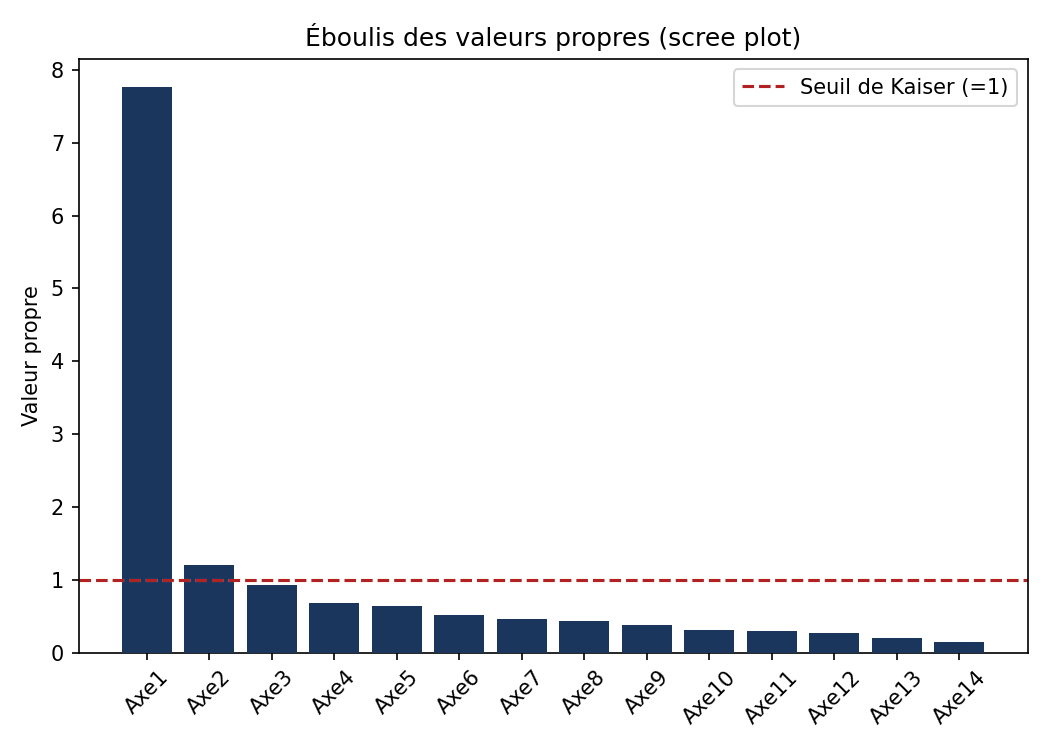
\includegraphics[width=\linewidth,height=5.50cm,keepaspectratio]{prism-uploads/graph4_eboulis_acp_bleu_fonce.png}\par
      \vspace{0.08cm}
      {\scriptsize\itshape Source : ANACIM, calculs de l’auteur.}
    \column{0.45\textwidth}
      \small
      \begin{itemize}
        \setlength\itemsep{0.32cm}
        \item Deux axes avec $\lambda>1$ : {\color{marine}\bfseries 7,76} et {\color{marine}\bfseries 1,20}.
        \item Variance expliquée : {\color{marine}\bfseries 54,6\%} (axe 1) et 8,4\% (axe 2), soit {\color{marine}\bfseries 63,0\%} cumulés.
        \item Chute nette entre les axes 1 et 2, puis décroissance progressive.
      \end{itemize}
  \end{columns}
\end{frame}

% 17. Résultats : interprétation des axes
\begin{frame}{Résultats (7/9) : interprétation des axes}
  \begin{columns}[T,onlytextwidth]
    \column{0.45\textwidth}
      \centering
      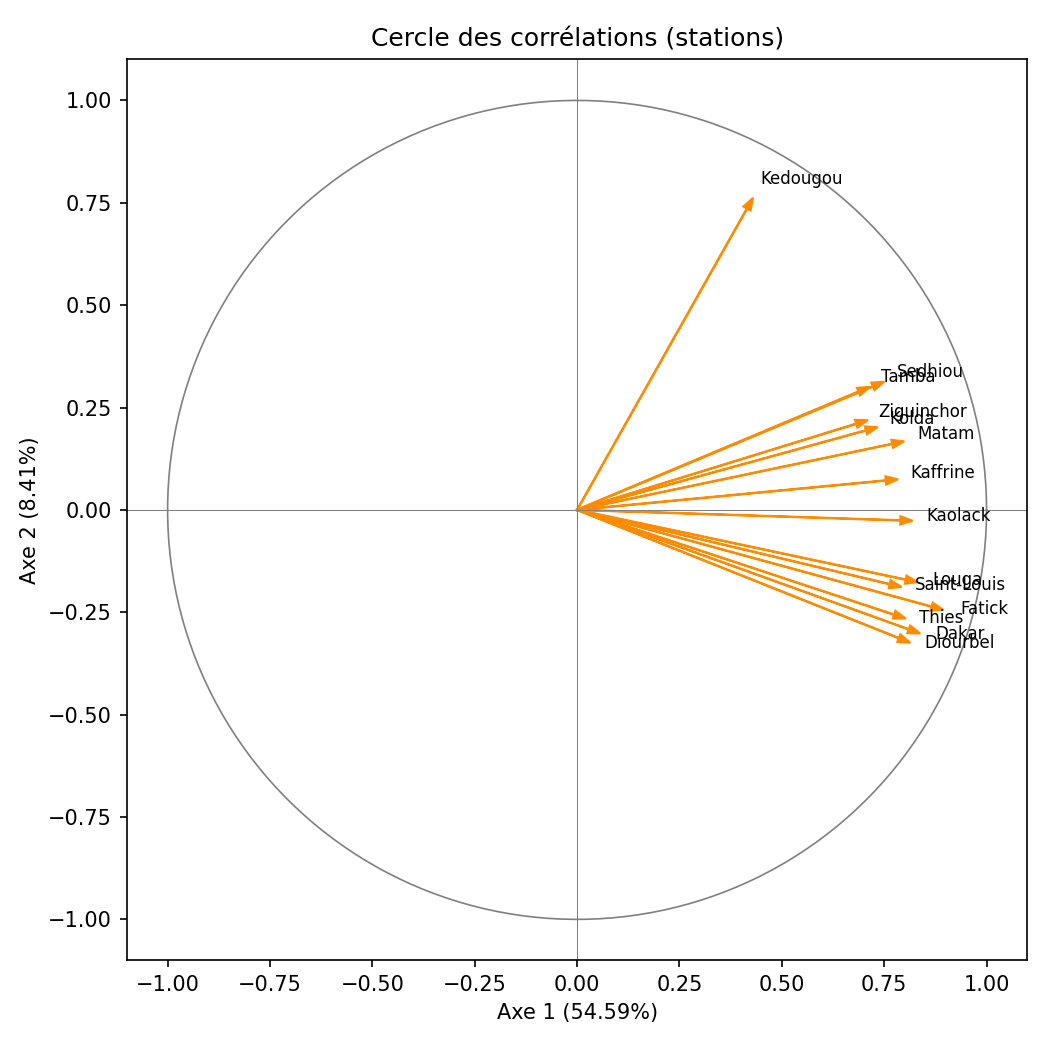
\includegraphics[width=\linewidth,height=5.50cm,keepaspectratio]{prism-uploads/graph5_cercle_correlations.png}\par
      \vspace{0.12cm}
      {\scriptsize\itshape Source : ANACIM, calculs de l’auteur.}
    \column{0.52\textwidth}
      \begin{beamercolorbox}[wd=\linewidth,rounded=true,sep=0pt]{contextbody}
        \begin{beamercolorbox}[wd=\linewidth,ht=0.38cm,dp=0.08cm,leftskip=0.14cm]{contextheading}
          \bfseries Axe 1 : signal national
        \end{beamercolorbox}
        \begin{beamercolorbox}[wd=\linewidth,sep=0.12cm]{contextbody}
          \small
          Toutes les régions sont corrélées positivement à l’axe 1 (de $0{,}41$ pour Kédougou à $0{,}87$ pour Fatick). Une année élevée correspond à une année excédentaire partout.
        \end{beamercolorbox}
      \end{beamercolorbox}
      \vspace{0.18cm}
      \begin{beamercolorbox}[wd=\linewidth,rounded=true,sep=0pt]{contextbody}
        \begin{beamercolorbox}[wd=\linewidth,ht=0.38cm,dp=0.08cm,leftskip=0.14cm]{contextheading}
          \bfseries Axe 2 : contraste secondaire
        \end{beamercolorbox}
        \begin{beamercolorbox}[wd=\linewidth,sep=0.12cm]{contextbody}
          \small
          Il oppose l’Est et le Sud (Kédougou, Sédhiou, Tambacounda, Ziguinchor, Kolda, Matam) à l’Ouest (Dakar, Diourbel, Thiès, Fatick, Saint-Louis, Louga).\par
          \textcolor{marine}{Pas strictement latitudinal} : le contraste est surtout porté par Kédougou ($0{,}74$).
        \end{beamercolorbox}
      \end{beamercolorbox}
  \end{columns}
\end{frame}

% 18. Résultats : trois régimes pluviométriques
\begin{frame}{Résultats (8/9) : trois régimes pluviométriques}
  \begin{columns}[T,onlytextwidth]
    \column{0.51\textwidth}
      \centering
      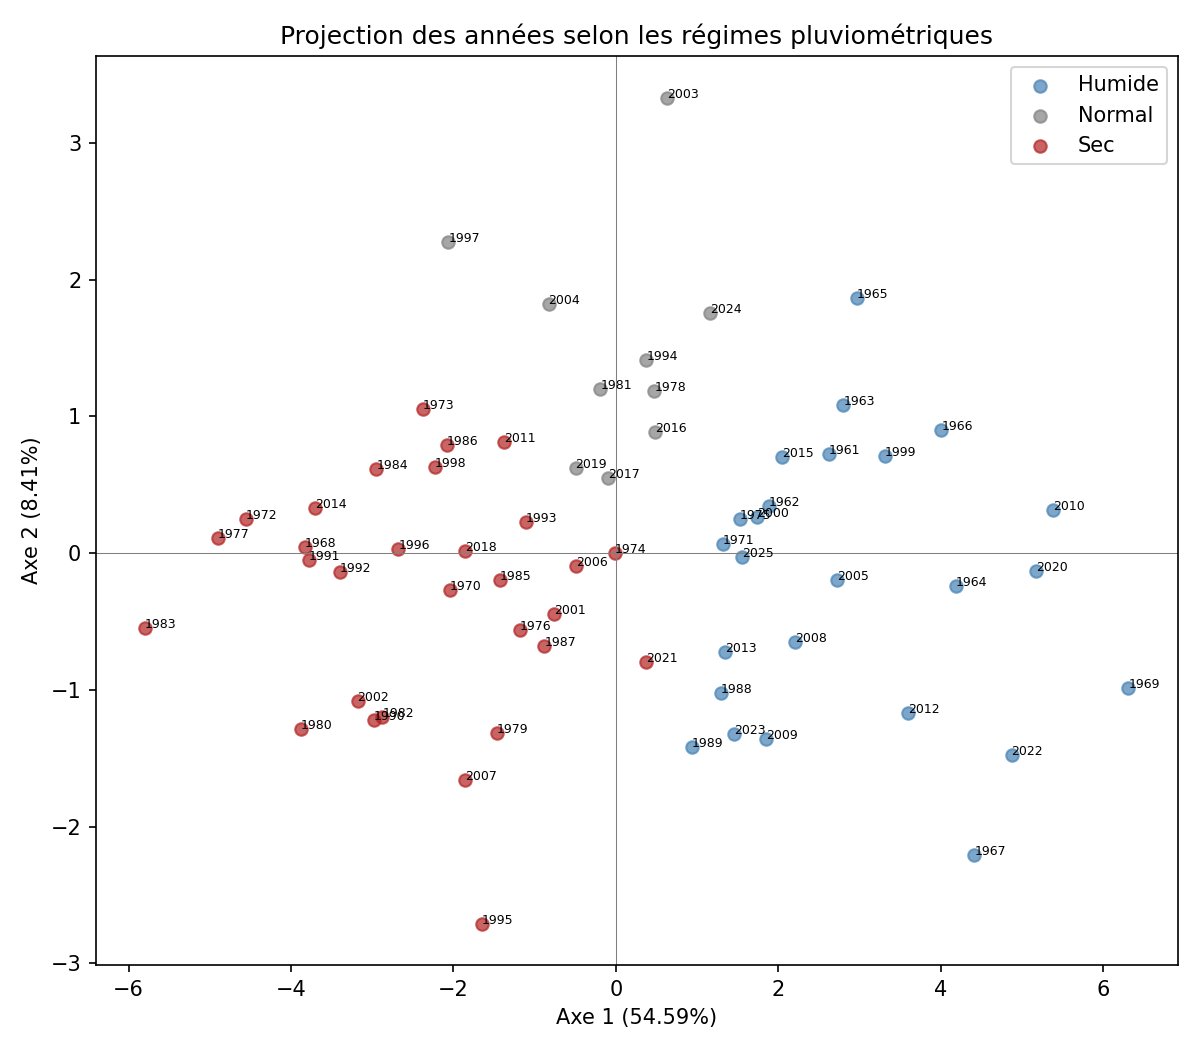
\includegraphics[width=\linewidth,height=5.50cm,keepaspectratio]{prism-uploads/graph6_projection_annees.png}\par
      \vspace{0.10cm}
      {\scriptsize\itshape Source : ANACIM, calculs de l’auteur.}
    \column{0.46\textwidth}
      \scriptsize
      \renewcommand{\arraystretch}{1.15}
      \setlength{\tabcolsep}{3pt}
      \begin{tabular*}{\linewidth}{@{\extracolsep{\fill}}lrrr@{}}
        \toprule
        \textbf{Régime} & \textbf{Années} & \textbf{Moy. (mm)} & \textbf{Min--Max}\\
        \midrule
        \textcolor{vertfonce}{Humide} & 25 & 823,2 & 717,7-977,8\\
        \textcolor{bleuvif}{Normal} & 10 & 714,3 & 635,7-799,2\\
        \textcolor{jauneregime}{Sec} & 30 & 584,9 & 418,2-692,2\\
        \bottomrule
      \end{tabular*}
      \vspace{0.12cm}
      \small
      \begin{itemize}
        \setlength\itemsep{0.12cm}
        \item Classes structurées par l’\textcolor{marine}{axe 1}.
        \item 1961-1967 : humide ; 1968-1987 : sec ; depuis 2008 : retour de l’humide, cohérent avec les ruptures.
        \item Le régime « normal » est une zone de transition.
      \end{itemize}
  \end{columns}
\end{frame}

% 19. Résultats : lecture régionale
\begin{frame}{Résultats (9/9) : lecture régionale, Dakar et Kédougou}
  \begin{columns}[T,onlytextwidth]
    \column{0.49\textwidth}
      \centering
      {\bfseries Dakar\par}
      \vspace{0.04cm}
      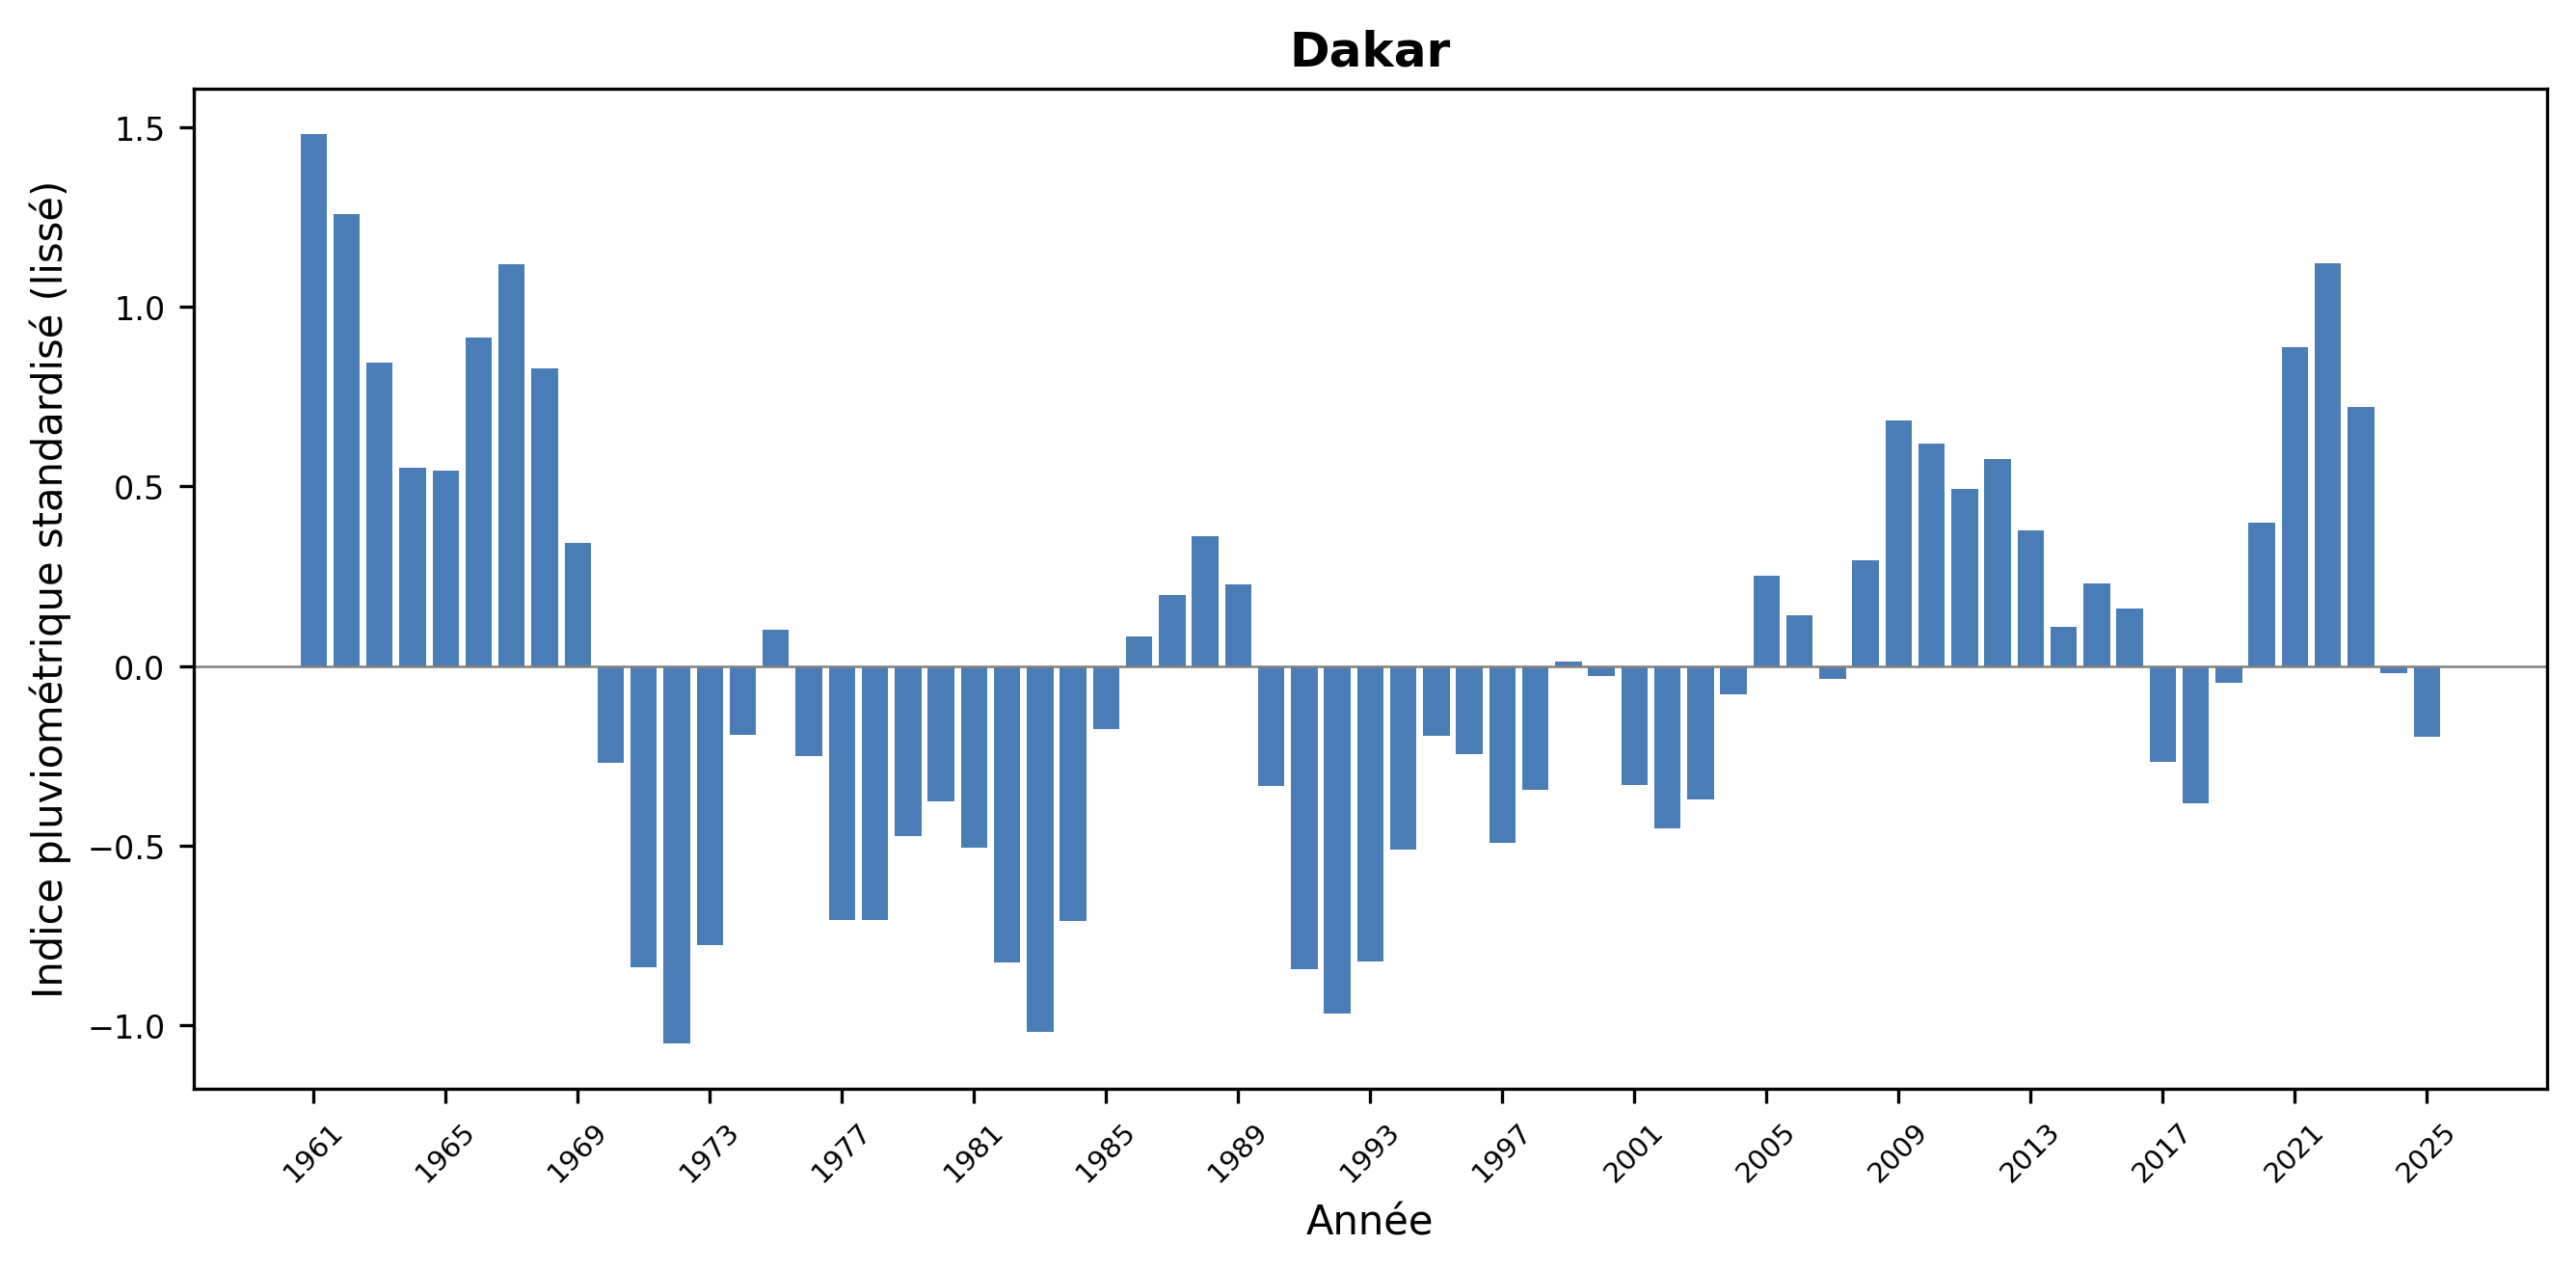
\includegraphics[width=\linewidth,height=3.20cm,keepaspectratio]{prism-uploads/Figure_IV4_3_Dakar.png}\par
      \vspace{0.05cm}
      {\scriptsize Reproduit les trois phases du signal national.}
    \column{0.49\textwidth}
      \centering
      {\bfseries Kédougou\par}
      \vspace{0.04cm}
      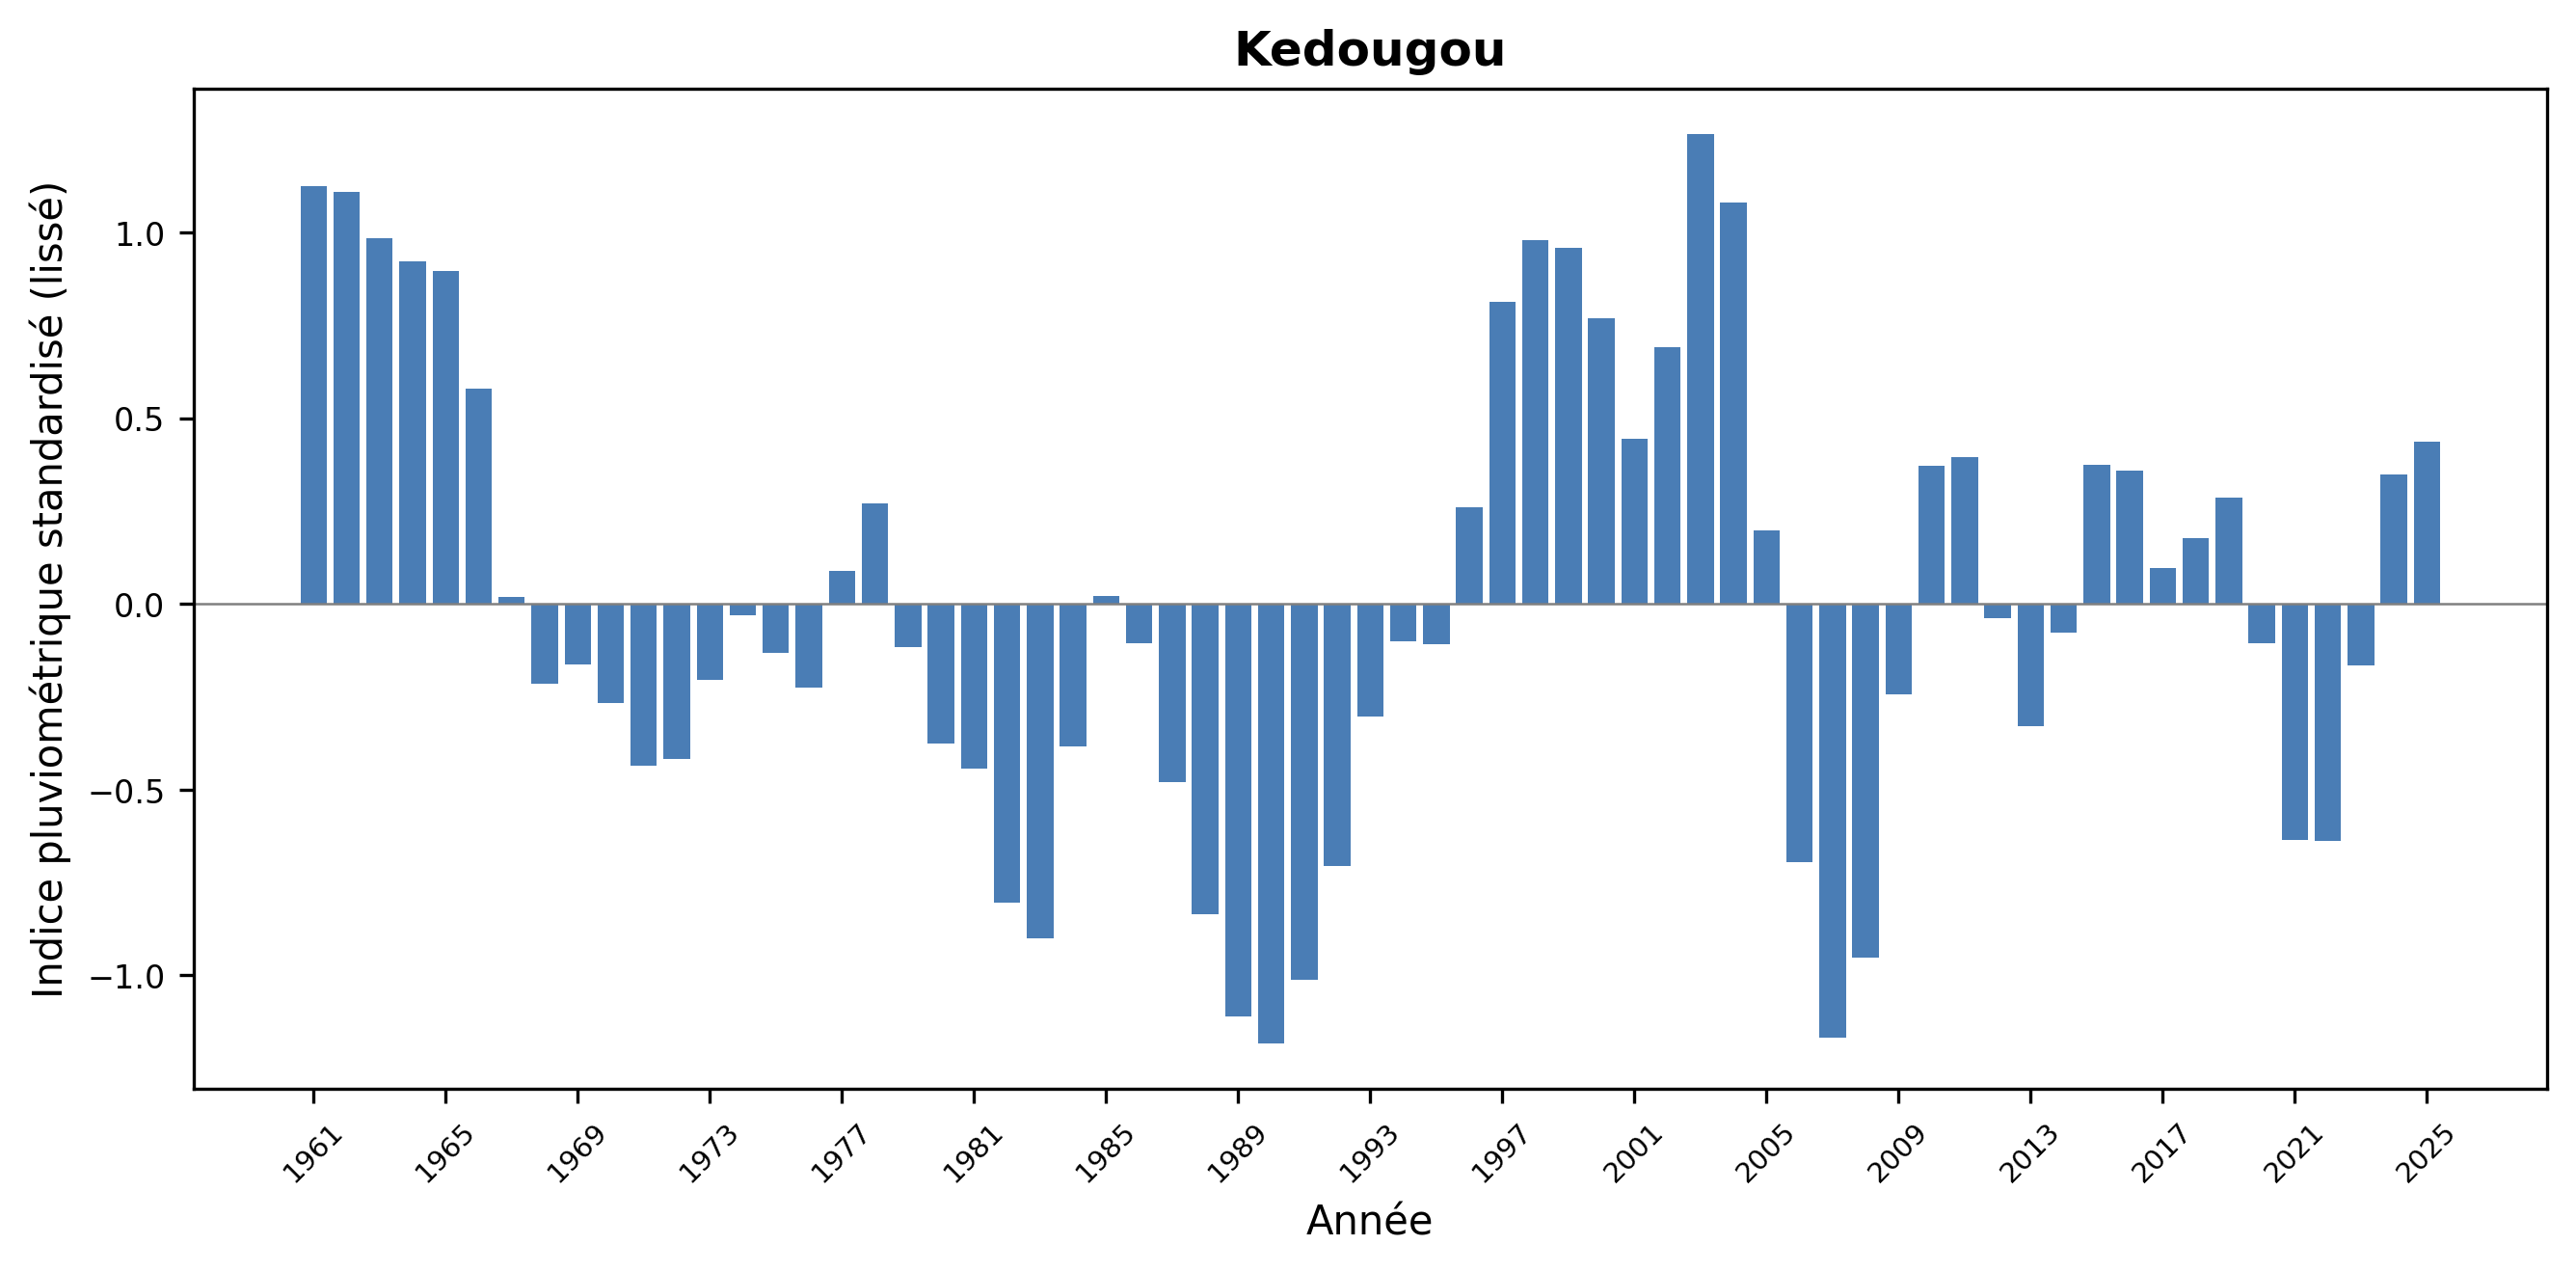
\includegraphics[width=\linewidth,height=3.20cm,keepaspectratio]{prism-uploads/Figure_IV4_3_Kedougou.png}\par
      \vspace{0.05cm}
      {\scriptsize Excédent marqué de 1991 à 2004, décalé par rapport au calendrier national.}
  \end{columns}
  \vspace{0.20cm}
  \centering\small IPS lissé (Hanning d’ordre 2) : appui visuel, pas un nouveau test.\par
  \vspace{0.12cm}
  {\centering\scriptsize\itshape Source : ANACIM, calculs de l’auteur.\par}
\end{frame}

% 20. Discussion : retour sur les hypothèses
\begin{frame}{Discussion (1/2) : retour sur les hypothèses}
  \vspace{0.48cm}
  \begin{center}
    \renewcommand{\arraystretch}{1.28}
    \begin{tabularx}{0.92\textwidth}{@{}>{\centering\arraybackslash\bfseries\color{marine}}m{0.55cm}>{\raggedright\arraybackslash}X>{\raggedright\arraybackslash\bfseries\color{marine}}m{2.50cm}@{}}
      H1 & Rupture significative : \textcolor{marine}{8 régions sur 14}, appuyées par $\geq 3$ procédures sur 4. & Confirmée \\[0.16cm]
      H2 & Moyennes avant/après différentes à 5\% dans les 8 régions concernées. & Confirmée \\[0.16cm]
      H3 & Hétérogénéité spatiale : l’axe 2 (8,4\%) oppose Est/Sud à l’Ouest, avec un rôle marqué de Kédougou. & Confirmée, nuancée \\[0.16cm]
      H4 & Trois classes interprétables recoupent les deux périodes de rupture ; le régime « normal » est une transition. & Confirmée, nuancée
    \end{tabularx}
  \end{center}
\end{frame}

% 21. Discussion : concordance avec la littérature
\begin{frame}{Discussion (2/2) : concordance avec la littérature}
  \begin{columns}[T,onlytextwidth]
    \column{0.49\textwidth}
      \begin{beamercolorbox}[wd=\linewidth,rounded=true,sep=0pt]{contextbody}
        \begin{beamercolorbox}[wd=\linewidth,ht=0.38cm,dp=0.08cm,leftskip=0.14cm]{contextheading}
          \bfseries Convergences
        \end{beamercolorbox}
        \begin{beamercolorbox}[wd=\linewidth,sep=0.08cm]{contextbody}
          \footnotesize
          \begin{itemize}
            \setlength\itemsep{0.04cm}
            \item Ruptures de 1966-1971 proches de Sagna et al. (2015), qui situent l’épisode entre \textcolor{marine}{1966 et 1969}.
            \item Résultats similaires à Gaye (2017) pour Saint-Louis, Podor et Matam.
            \item Baisses de 16 à 32\%, du même ordre que chez Bodian (2014), avec un maximum plus marqué à Dakar.
            \item Reprise des années 2000 également observée par Gaye (2017) et Diop (2023).
          \end{itemize}
        \end{beamercolorbox}
      \end{beamercolorbox}
    \column{0.49\textwidth}
      \begin{beamercolorbox}[wd=\linewidth,rounded=true,sep=0pt]{contextbody}
        \begin{beamercolorbox}[wd=\linewidth,ht=0.38cm,dp=0.08cm,leftskip=0.14cm]{contextheading}
          \bfseries Lecture
        \end{beamercolorbox}
        \begin{beamercolorbox}[wd=\linewidth,sep=0.08cm]{contextbody}
          \footnotesize
          \begin{itemize}
            \setlength\itemsep{0.07cm}
            \item Rupture des années 1960 : mise en perspective avec la mousson ouest-africaine et les conditions océaniques.
            \item Reprise \textcolor{marine}{partielle}, sans retour au régime antérieur.
            \item Apport : analyse conjointe des 14 régions sur 65 ans, ruptures et approche multivariée.
          \end{itemize}
        \end{beamercolorbox}
      \end{beamercolorbox}
  \end{columns}
  \vspace{0.16cm}
  \begin{beamercolorbox}[wd=\textwidth,rounded=true,sep=0pt]{contextbody}
    \begin{beamercolorbox}[wd=\linewidth,ht=0.36cm,dp=0.08cm,leftskip=0.14cm]{contextheading}
      {\color{marine}\bfseries Cas à part}
    \end{beamercolorbox}
    \begin{beamercolorbox}[wd=\linewidth,sep=0.09cm]{contextbody}
      \footnotesize Kaolack (tendance progressive) et Matam (autocorrélation) : l’absence de rupture validée est cohérente avec ces anomalies.
    \end{beamercolorbox}
  \end{beamercolorbox}
\end{frame}

% 22. Conclusion : synthèse des résultats
\begin{frame}{Conclusion : ce qu’il faut retenir}
  \vspace{0.42cm}
  \begin{columns}[T,onlytextwidth]
    \column{0.32\textwidth}
      \begin{beamercolorbox}[wd=\linewidth,rounded=true,sep=0pt]{contextbody}
        \begin{beamercolorbox}[wd=\linewidth,ht=0.46cm,dp=0.08cm,leftskip=0.14cm]{contextheading}
          \bfseries Ruptures
        \end{beamercolorbox}
        \par\vspace{0.22cm}
        \begin{beamercolorbox}[wd=\linewidth,sep=0.14cm]{contextbody}
          \small
          \vspace*{0.22cm}
          \linespread{1.08}\selectfont
          \textcolor{marine}{8 régions sur 14} : chute de $-16$ à $-32\%$ (1966-1971), puis hausse de $+17$ à $+23\%$ (1998-2007).
        \end{beamercolorbox}
      \end{beamercolorbox}
    \column{0.32\textwidth}
      \begin{beamercolorbox}[wd=\linewidth,rounded=true,sep=0pt]{contextbody}
        \begin{beamercolorbox}[wd=\linewidth,ht=0.46cm,dp=0.08cm,leftskip=0.14cm]{contextheading}
          \bfseries Structure spatiale
        \end{beamercolorbox}
        \par\vspace{0.22cm}
        \begin{beamercolorbox}[wd=\linewidth,sep=0.14cm]{contextbody}
          \small
          \vspace*{0.22cm}
          \linespread{1.08}\selectfont
          Un signal national (54,6\%) et un contraste Est/Sud--Ouest secondaire, porté par Kédougou.
        \end{beamercolorbox}
      \end{beamercolorbox}
    \column{0.32\textwidth}
      \begin{beamercolorbox}[wd=\linewidth,rounded=true,sep=0pt]{contextbody}
        \begin{beamercolorbox}[wd=\linewidth,ht=0.46cm,dp=0.08cm,leftskip=0.14cm]{contextheading}
          \bfseries Régimes
        \end{beamercolorbox}
        \par\vspace{0.22cm}
        \begin{beamercolorbox}[wd=\linewidth,sep=0.14cm]{contextbody}
          \small
          \vspace*{0.22cm}
          \linespread{1.08}\selectfont
          \textcolor{marine}{25 années humides, 10 normales et 30 sèches}, en cohérence avec les ruptures.\par\vspace{0.40cm}
        \end{beamercolorbox}
      \end{beamercolorbox}
  \end{columns}
  \vspace{0.35cm}
  \begin{beamercolorbox}[wd=\textwidth,rounded=true,sep=0pt]{contextbody}
    \begin{beamercolorbox}[wd=\linewidth,ht=0.40cm,dp=0.08cm,leftskip=0.14cm]{contextheading}
      \bfseries Limites de l’étude
    \end{beamercolorbox}
    \begin{beamercolorbox}[wd=\linewidth,sep=0.12cm]{contextbody}
      \footnotesize
      Échelle régionale et cumuls annuels uniquement ; règle de $\pm 3$ ans choisie pour l’étude (sensibilité en annexe) ; Kaolack et Matam testées malgré leurs anomalies ; axe 2 à peine au-dessus du seuil de Kaiser ; trois classes fixées a priori.
    \end{beamercolorbox}
  \end{beamercolorbox}
\end{frame}

% 23. Recommandations
\begin{frame}{Recommandations et perspectives}
  \vspace{0.38cm}
  \begin{columns}[T,onlytextwidth]
    \column{0.48\textwidth}
      \begin{beamercolorbox}[wd=\linewidth,rounded=true,sep=0pt]{contextbody}
        \begin{beamercolorbox}[wd=\linewidth,ht=0.42cm,dp=0.10cm,leftskip=0.16cm]{contextheading}
          \bfseries Pour les institutions
        \end{beamercolorbox}
        \par\vspace{0.08cm}
        \begin{beamercolorbox}[wd=\linewidth,sep=0.12cm]{contextbody}
          \small
          \begin{itemize}
            \setlength\itemsep{0.16cm}
            \item \textcolor{marine}{Densifier le réseau pluviométrique} et renforcer le contrôle d’homogénéité des séries.
            \item Créer un système national de statistiques environnementales.
            \item Intégrer ces séries aux outils de planification.
          \end{itemize}
        \end{beamercolorbox}
      \end{beamercolorbox}
    \column{0.48\textwidth}
      \begin{beamercolorbox}[wd=\linewidth,rounded=true,sep=0pt]{contextbody}
        \begin{beamercolorbox}[wd=\linewidth,ht=0.42cm,dp=0.10cm,leftskip=0.16cm]{contextheading}
          \bfseries Pour la recherche
        \end{beamercolorbox}
        \par\vspace{0.08cm}
        \begin{beamercolorbox}[wd=\linewidth,sep=0.12cm]{contextbody}
          \small
          \begin{itemize}
            \setlength\itemsep{0.12cm}
            \item Exploiter les données \textcolor{marine}{infra-annuelles} : saison des pluies, nombre de jours pluvieux et intensité des épisodes.
            \item Développer des modèles prédictifs et relier les résultats aux données hydrologiques et agricoles pour éclairer les impacts et la prévision.
            \item Prolonger les séries, en contrôler l’homogénéité et les comparer à CHIRPS et GPCC.
          \end{itemize}
        \end{beamercolorbox}
      \end{beamercolorbox}
  \end{columns}
\end{frame}

% 15. Remerciements
\begin{frame}[plain]
  \begin{tikzpicture}[remember picture,overlay]
    \fill[white] (current page.south west) rectangle (current page.north east);
    \draw[marine,line width=0.8pt] ([xshift=0.12cm,yshift=-0.12cm]current page.north west) circle (0.82cm);
    \draw[or,line width=0.8pt] ([xshift=0.12cm,yshift=-0.12cm]current page.north west) circle (1.02cm);
    \draw[marine,line width=0.8pt] ([xshift=-0.12cm,yshift=0.12cm]current page.south east) circle (0.82cm);
    \draw[or,line width=0.8pt] ([xshift=-0.12cm,yshift=0.12cm]current page.south east) circle (1.02cm);
    \draw[or,line width=1.1pt] (current page.south west) -- ([xshift=\paperwidth]current page.south west);
    \draw[marine,line width=2.2pt] ([yshift=0.08cm]current page.south west) -- ([xshift=\paperwidth,yshift=0.08cm]current page.south west);
  \end{tikzpicture}
  \vfill
  \begin{center}
    {\color{marine}\LARGE\bfseries MERCI POUR VOTRE ATTENTION.\par}
    \vspace{0.10cm}
    {\color{or}\rule{0.37\linewidth}{1.2pt}\par}
  \end{center}
  \vfill
\end{frame}

\end{document}